% Pole and polar: the polar of P is the chord of contact T1T2; on every secant, (M,N;P,Q) = -1.
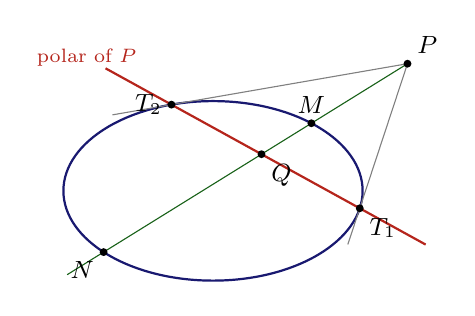
\begin{tikzpicture}[scale=0.95,font=\small]
\draw[MidnightBlue,thick] (0,0) ellipse (2.0000 and 1.2000);
\draw[black!50] (2.6000,1.7000) -- (1.8024,-0.7164) (2.6000,1.7000) -- (-1.3442,1.0160);
\draw[BrickRed,thick] (2.8429,-0.7182) -- (-1.4364,1.6379);
\draw[ForestGreen!70!black] (2.6000,1.7000) -- (-1.9498,-1.1209);
\fill (2.6000,1.7000) circle (1.5pt) node[above right] {$P$};
\fill (1.9619,-0.2331) circle (1.5pt) node[below right] {$T_1$};
\fill (-0.5553,1.1528) circle (1.5pt) node[left] {$T_2$};
\fill (1.3157,0.9038) circle (1.5pt) node[above] {$M$};
\fill (-1.4623,-0.8186) circle (1.5pt) node[below left] {$N$};
\fill (0.6484,0.4900) circle (1.5pt) node[below right] {$Q$};
\node[BrickRed,font=\scriptsize] at (-1.6881,1.7765) {polar of $P$};
\end{tikzpicture}
